% Prose body of the paper. Edit this (on Overleaf) for the actual writing.
% paper.tex \input{}s this for the styled LaTeX PDF; build-md.sh converts THIS file
% (pandoc) into the body of paper.md for JOSS. Keep it to sections + math + \citep so
% the LaTeX->Markdown conversion stays clean (no title/sidebar/preamble here).

\section{Summary}

\texttt{jspsych-ado} brings browser-native \emph{adaptive design optimization} (ADO) to behavioral experiments built with jsPsych \citep{deleeuw2015jspsych}.
After each response, a Bayesian model written in Stan \citep{carpenter2017stan} --- compiled to WebAssembly and run client-side in a Web Worker --- updates the posterior over the model parameters, and the next stimulus is chosen to maximize the expected information it provides about those parameters.
Because the adaptive loop runs entirely in the participant's browser, experiments can be deployed as static web assets rather than server-backed applications.
The package separates task presentation, response-model specification, and adaptive control so that new tasks and models can be implemented without rewriting the inference-and-design engine.

\section{Statement of need}

Many behavioral experiments use fixed stimulus schedules even when some trials are more informative than others for estimating model parameters or discriminating among theoretical accounts. 
Adaptive design optimization (ADO) addresses this problem by treating stimulus selection as a sequential Bayesian design problem: after observing a response, the experimenter updates uncertainty about the model and selects the next design expected to provide the most information \citep{cavagnaro2010adaptive,myung2013tutorial}. 
Applications to delay-discounting measurement, risky-choice model discrimination, and mnemonic-similarity testing show that ADO is useful across behavioral domains where participant time is limited and informative trials are valuable \citep{ahn2020rapid,cavagnaro2012optimal,villarreal2022adaptive}. 
However, using ADO in practice requires researchers to connect experimental presentation, response modeling, Bayesian updating, and design selection within the same data-collection workflow.

This integration is especially challenging for browser-based behavioral experiments. jsPsych has made it possible to build flexible online experiments with response-contingent timelines, reusable plugins, and simulation tools for testing experiment logic \citep{deleeuw2023jspsych}. 
However, jsPsych does not provide a general model-based ADO layer: researchers must still implement or connect the model likelihood, posterior update, and next-stimulus selection logic for each adaptive experiment.
As a result, applying ADO in browser studies typically requires custom glue code that is difficult to reuse, inspect, and validate across tasks.

Existing adaptive-design tools address important parts of this problem but do not provide this combination of capabilities for jsPsych experiments. 
ADOpy lowers the barrier to ADO through a modular Python implementation \citep{yang2021adopy}, while QUEST+ and jsQuestPlus support adaptive psychophysical procedures, including browser-based use \citep{watson2017questplus,kuroki2022jsquestplus}. 

These tools demonstrate the value of accessible adaptive experimentation, but they do not provide a jsPsych-native layer that couples task presentation, Bayesian response models, posterior updating, and information-based stimulus selection inside the browser experiment itself.
\texttt{jspsych-ado} fills this gap by separating task, model, and controller components so that researchers can implement adaptive browser experiments without rewriting the inference-and-design engine for each new task.
% TODO: expand with the concrete use cases and who benefits.
%clinicnal settings? automated testing?

\section{State of the field}

Advances in statistics and machine learning have offered algorithm-based ways to identify principled experimental designs decision based on information gain \citep{watson1983quest,cavagnaro2010adaptive,rainforth2024modern,huan2024optimal}. 
Specifically relevant to our approach, Bayesian experimental design is a
model-based approach to designing optimal experiments. We start with a Bayesian
model $p(\theta)\,p(y \mid d, \theta)$ of the underlying process we are interested
in. The model has parameters $\theta$ with prior $p(\theta)$: these are the
quantities we would like to learn or infer. The data model $p(y \mid d, \theta)$
describes how the data $y$ are generated given the parameters $\theta$ and the
design $d$.

The optimal design $d^{*}$ is the one that maximises the expected information
gain (EIG) about the parameters $\theta$. The EIG is the expected reduction in
Shannon entropy from the prior $p(\theta)$ to the posterior $p(\theta \mid y, d)$
that results from the experiment with design $d$:
%
\begin{equation}
d^{*} = \arg\max_{d}\; \mathrm{EIG}(d),
\qquad
\mathrm{EIG}(d)
  = \mathbb{E}_{p(y \mid d)}\!\Big[\, H\big(p(\theta)\big) - H\big(p(\theta \mid y, d)\big) \,\Big],
\label{eq:eig}
\end{equation}
%
where $H(\cdot)$ is the Shannon entropy and the expectation is taken over the
prior predictive distribution $p(y \mid d) = \int p(y \mid d, \theta)\,p(\theta)\,\mathrm{d}\theta$.


In general optimal design based on a mutual-information formulation like these are used in a variety of fields such as XXX CITE and YYY CITE they are widely used in psychophysics \citep{watson2017questplus}, XXX and more resently psychiaary XXX. With software implemetnations being brought (e.g.\ PyBOLE
\citep{myrodia2026pybole}), ADOpy \citep{yang2020adopy}, and jsQuestPlus \citep{kuroki2023jsquestplus}

While running Stan in the browser via WebAssembly was recently demonstrated\citep{stanplayground}, but it has not been used for applicaitons like adaptive design. \texttt{jspsych-ado} combines in-browser inference with mutual-information design optimization inside the jsPsych ecosystem.

% Can refer to https://github.com/githubpsyche/jspsych-ado/issues/35 for other possibly useful references

\section{Software design}

Figure~\ref{fig:conceptual} summarizes the runtime loop implemented by \texttt{jspsych-ado}.
On each trial, the controller scores candidate designs and selects the one expected to provide the most information.
jsPsych then presents the selected design and records the participant's response.
The inference backend uses the accumulated responses and registered model to update the posterior distribution over parameters.
Candidate designs are the stimulus settings the controller can choose from, such as reward and delay values in a delay-discounting task or line lengths in a psychophysical task.

\begin{figure}
    \centering
    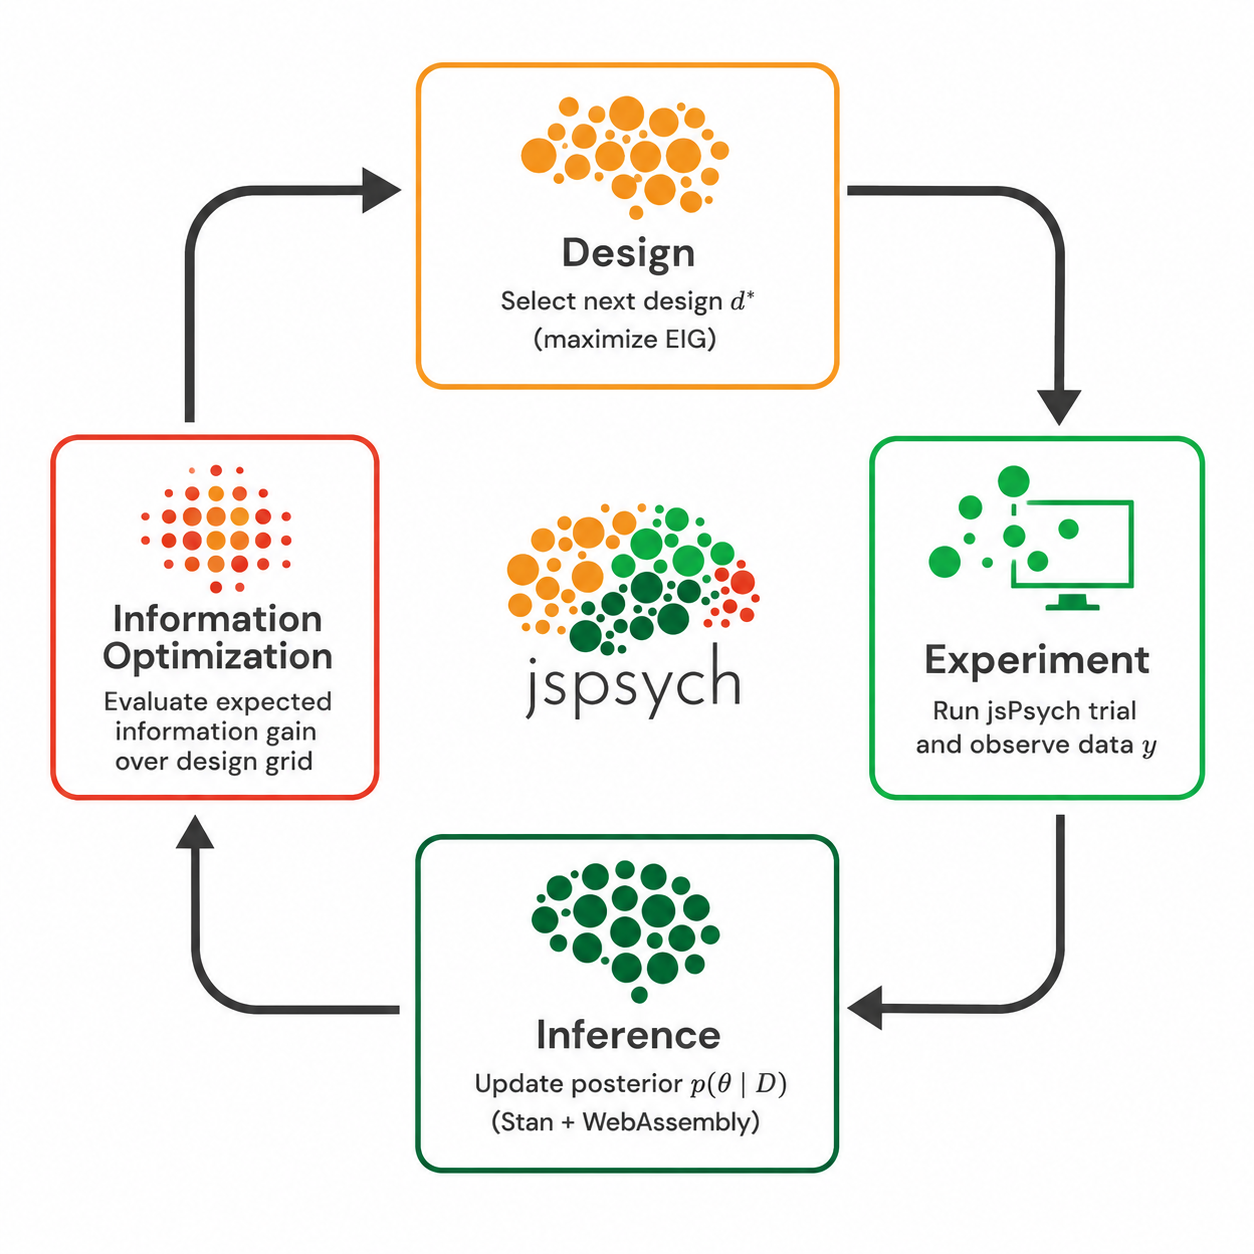
\includegraphics[width=0.75\linewidth]{paper//figures/jspsych-ado-conceptual.png}
    \caption{Conceptual loop implemented by \texttt{jspsych-ado}. Candidate designs are scored by expected information gain, the selected design is presented as a jsPsych trial, the participant's response is used to update the posterior, and the updated posterior informs the next design selection.}
    \label{fig:conceptual}
\end{figure}

Figure~\ref{fig:code-block} shows how this loop is exposed to users.
An experiment registers a task and a model, then calls \texttt{createTimeline} to construct the adaptive jsPsych timeline.
Tasks own the participant-facing pieces: candidate designs, display logic, response options, and response coding.
A model owns the statistical response process.
A controller connects the registered task and model, checks that their design variables and response spaces are compatible, and chooses designs during the experiment.
This separation lets researchers change the participant-facing task, the statistical model, or the adaptive policy independently.

The model package defines the statistical quantities that the controller needs for inference and design scoring.
The adaptive loop requires two statistical computations.
First, after each response, the system must update uncertainty about model parameters; this is Stan's role.
The registered Stan model is fit to the accumulated trial history, and the controller receives posterior draws from \(p(\theta \mid D)\).
Second, the system must predict how a participant would respond to each candidate design under possible parameter values.
This is the role of the model's JavaScript \texttt{responseProb} or \texttt{responseProbs} function, which the controller evaluates over the design grid.
A model package therefore supplies parameter names and priors, Stan code or a compiled WebAssembly artifact, the data mapping from jsPsych trial rows to Stan input, and the JavaScript response-probability function.

The Stan controller scores each candidate design by the expected information
gain defined above, applied at every trial with the current posterior
$p(\theta \mid D)$ in place of the prior. Stan then supplies the posterior draws
$\theta^{(s)} \sim p(\theta \mid D)$, while the model's response-probability function supplies the likelihood $p(y \mid d, \theta)$. Because mutual information is only the entropy of the posterior-predictive response minus the expected entropy of the per-draw response, the controller evaluates the mathrm{EIG} in a relatively sparse response space (binary or a few categories) making the computation inexpensive. It computes this over the task's finite design grid $\mathcal{G}$ and selects the highest-scoring design $d^{*}$ for the next trial.

Running posterior inference in the browser makes deployment simpler, but also sets practical limits on model complexity and per-trial update time.
Stan models must be compiled before they can run in the browser; models bundled with \texttt{jspsych-ado} include these compiled WebAssembly files.
Users developing new models can compile from Stan source during setup, including through the stan-playground compile server \citep{stanplayground,zakai2011emscripten}.
At runtime, sampling runs in a Web Worker so posterior updates do not block the participant-facing interface.
The current implementation therefore targets browser-feasible Stan models, finite design grids, and finite binary or categorical response spaces rather than continuous online design optimization.

The same interfaces also support validation. 
Simulated participants and the mutual-information engine call the same JavaScript response-probability function, so browser simulation can exercise the same jsPsych timeline used in a live experiment without maintaining a separate data generator.
The resulting recovery, parity, and browser-level checks are discussed below as evidence of research impact.

\section{Example: adaptive numerosity discrimination}
\begin{figure}
    \centering
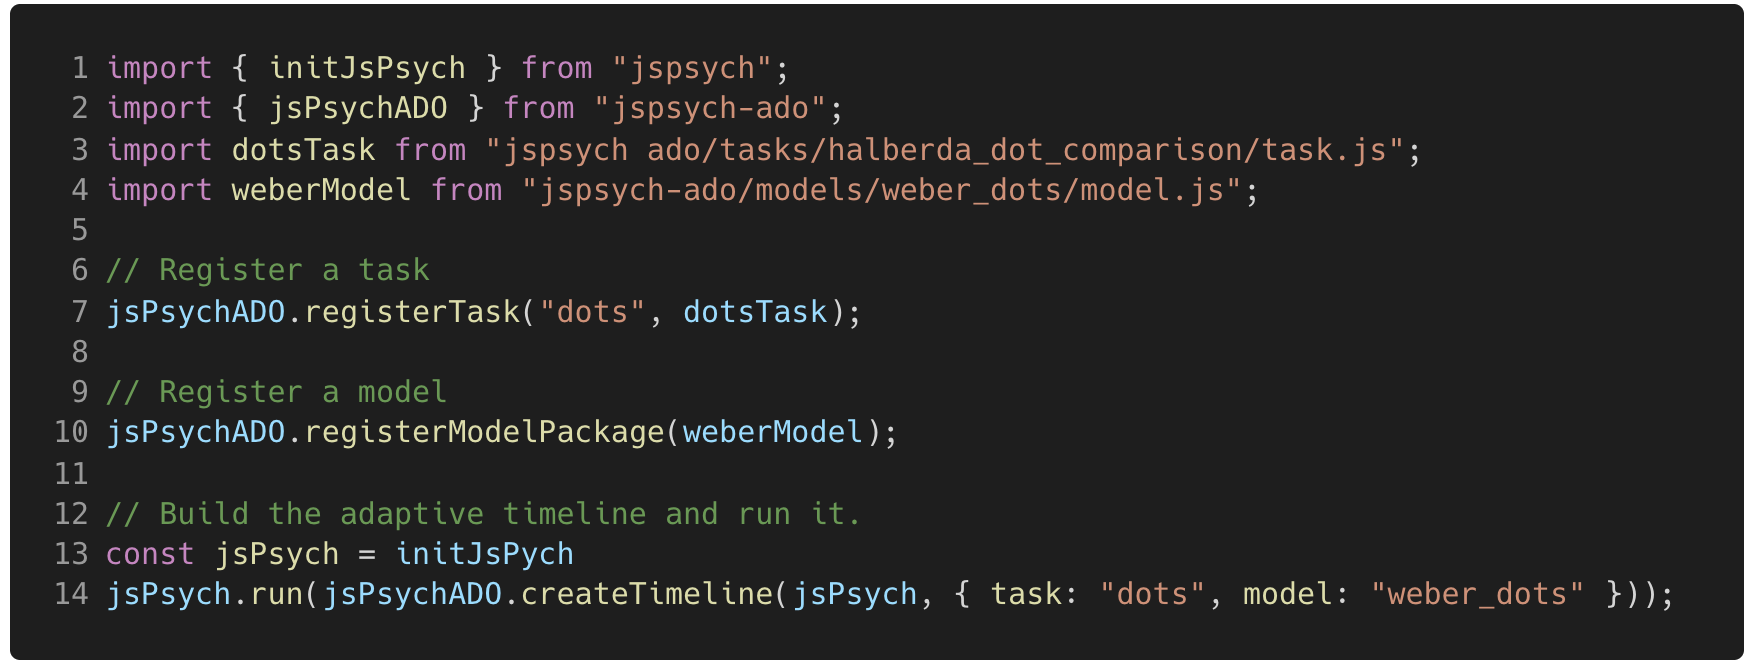
\includegraphics[width=1\linewidth]{paper//figures/jspsych-ado-code_block.png}
    \caption{Minimal \texttt{jspsych-ado} workflow. Users register a task that defines the stimuli and responses, register a model that defines the statistical response process, and create an adaptive jsPsych timeline from the paired task and model.}
\label{fig:code-block}
\end{figure}

We will now explain the details using a numerosity (numeric) discrimination task, following \citet{halberda2008individual}, which ships with the package as a ready-to-run task/model pair. In this example there is a single stimulus parameter controling the numerosity ratio of the two dot arrays and denoted by the design $d$ and a single model parameter, the Weber fraction $\theta = w$ (a participant's approximate-number-system acuity). A cumulative-normal (probit) function $\Phi$ is assumed to be the psychometric function, and the task is two-alternative forced choice (the participant judges which color is more numerous), giving a binary response $y$. Using the ADO method, the Weber fraction can be estimated, with the next dot pair $d^{*}$ on each trial
chosen to maximize the expected information gain about $w$.

After $t$ trials, the accumulated dataset is $D = \{(d_i, y_i)\}_{i=1}^{t}$, and Stan samples the posterior over $\theta$:
%
\[
  p(\theta \mid D) \;\propto\; p(\theta)\,\prod_{i=1}^{t} p(y_i \mid d_i, \theta).
\]
%
The probit psychometric function gives the probability of a correct response as
%
\[
  p(Y = 1 \mid d, \theta)
  = \Phi\!\left(\frac{n_{\text{large}} - n_{\text{small}}}
                     {w\,\sqrt{n_{\text{large}}^{2} + n_{\text{small}}^{2}}}\right),
\]
%
where $n_{\text{large}}$ and $n_{\text{small}}$ are the larger and smaller dot
counts in design $d$. The next design then maximizes the $\mathrm{EIG}(d)$, evaluated under the current posterior $p(\theta \mid D)$ and estimated by Monte Carlo over the posterior draws $\theta^{(s)} \sim p(\theta \mid D)$:
%
\[
  d^{*} = \arg\max_{d \in \mathcal{G}}\; I(\Theta; Y \mid d, D)
        = H\!\big(\bar{p}_d\big)
          - \frac{1}{S}\sum_{s=1}^{S} H\!\big(p(Y \mid d, \theta^{(s)})\big),
  \qquad
  \bar{p}_d = \frac{1}{S}\sum_{s=1}^{S} p(Y \mid d, \theta^{(s)}),
\]
%
where $\bar{p}_d$ is the Monte-Carlo estimate of the posterior-predictive response probability $p(Y \mid d, D)$. This is exactly what the engine's design-selection routine computes from the posterior draws.

\section{Research impact statement}

Prior ADO software has emphasized that implementation demands limit broader use of adaptive design methods \citep{yang2021adopy}.
\texttt{jspsych-ado} addresses the same problem for browser experiments by providing reusable jsPsych components for posterior updating, information-based design selection, and adaptive timeline construction.
It is distributed through npm, documented with runnable examples, and organized around shareable task and model packages.
The included examples span delay discounting, line-length psychophysics, and approximate-number discrimination; additional examples show how to add a new task or a new model through the same interface.
This structure provides a common scaffold for collaborative development within the jsPsych ecosystem.
The validation materials exercise the browser workflow directly: simulated participants run through the same jsPsych pages used in live studies, parameter-recovery examples compare information-based designs with random designs from the same candidate grid, and likelihood-parity checks compare the JavaScript and compiled Stan likelihoods.
Continuous integration covers unit tests, browser smoke tests, Worker/WebAssembly execution, and bundler compatibility, supporting reuse by researchers who want to inspect, extend, and share adaptive jsPsych experiments.

Because the nontrivial technical skills required to use ADO have been a barrier to its wider adoption, we believe jsPsych-ADO will positively impact the integration of adaptive designs across a broader range of tasks in the social and behavioral sciences. It lowers the barrier to entry for including an adaptive version of a task by eliminating the need to write bespoke adaptive design code, while offering implementations across a range of existing tasks and computational models used in prior work on adaptive designs, such as delay discounting \citep{lee2026rapid} and numeric discrimination \citep{halberda2008individual}. Further, it enhances collaboration by providing researchers with a shared scaffold for developing and sharing new adaptive designs within a common ecosystem (i.e., jsPsych). We aim to continue developing jsPsych-ADO and extend its capabilities beyond those of existing implementations for adaptive experimental design.

\section{AI usage disclosure}
Generative AI tools were used during the development of jspsych-ado. Claude Code and OpenAI Codex assisted with code implementation, automating the release workflow, and providing code reviews during pull requests. All AI-generated content was reviewed and edited by the authors to ensure accuracy and clarity.
\section{Acknowledgements}
We thank the jsPsych Summer Hackathon participants for their support and feedback.

